\documentclass[letterpaper]{article}
\usepackage{aaai20}
\usepackage{times}
\usepackage{helvet}
\usepackage{courier}
\usepackage[hyphens]{url}
\usepackage{graphicx}
\urlstyle{rm}
\def\UrlFont{\rm}
\usepackage{graphicx}
\frenchspacing
\setlength{\pdfpagewidth}{8.5in}
\setlength{\pdfpageheight}{11in}

\newcommand{\ct}[1]{\texttt{#1}}


\pdfinfo{
    /Title (CSE579: Automated Fulfillment Warehouse Case Study - Project Report)
    /Author (Youmi Koh)
}

\title{

    Answer Set Programming Model for \\
    Automated Fulfillment Warehouse\\


}
\author{
    Written by Youmi Koh \\
    Arizona State University \\
    ykoh7@asu.edu
}
\date{July 3, 2023}

\begin{document}

\maketitle

\begin{abstract}
This report presents the Automated Fulfillment Warehouse Scenario and its representation as a planning problem using Answer Set Programming. It provides background on the methodology used in encoding the scenario, and discusses the results from solving the program using clingo. The report highlights critical constraints for producing valid and optimal plans, and highlights opportunities for future work.
\end{abstract}

\section{Problem Statement}

\noindent The Automated Fulfillment Warehouse Scenario illustrates a warehouse environment staffed with robots that are tasked with delivering products on stock shelves to appropriate picking stations where orders are fulfilled. Orders can be composed of multiple product line items, and robots have various operational limitations. The objective is to devise a plan that fulfills all warehouse orders in the least number of time steps.


\section{Project Background}

\noindent The Automated Warehouse Scenario is a planning problem that can be represented using answer set programming (ASP), a declarative programming paradigm that models problems as logic programs, and represents them as a set of rules and constraints. The variables of the program are instantiated with values to produce a grounded program, which serves as the program's knowledge base for deducing the universe of solutions. ASP solvers ground programs, then compute answer sets, which consists of atoms that satisfy all rules and constraints of the program.

Rules and constraints are expressed using fluents, actions, and axioms. Fluents depict the state of the world at a given time, and can be influenced by actions and axioms. Actions are the events that can occur in the world, and can affect the state of the world. Axioms are the rules that govern the behaviour of the world, and can be used to constrain the state of the world and the actions that can occur. The program's solution space is reduced to produce a set of answer sets that satisfy all rules and constraints of the program.

Programs for planning problems are encoded with a starting state and a future goal state. An objective function is defined to evaluate the quality of a plan, and the aim finding plans that transforms the starting state into the goal state while optimizing the objective function.

In this scenario, the program is initialized with a starting instance state for all components of the warehouse, and the goal state is defined as a warehouse with all orders fulfilled. The makespan function is expressed as the number of time steps required to fulfill all orders, and optimal plans minimize the makespan value. In this project, we will use clingo as the ASP solver, to find these optimal plans.


\section{Program Representation and Methodology}

Inside the warehouse, the scenario starts at time \ct{T=0} and the floor is represented in a grid format. Every cell on the grid floor is expressed as \ct{node(N,(X,Y))} where \ct{(X,Y)} are the cell coordinates, and symbolize a location of the warehouse floor where physical objects can be positioned. Certain cells of the warehouse floor are designated as highways and order picking stations, expressed as \ct{highway(H,(X,Y))} and \ct{pickingStation(PS,(X,Y))} respectively.

All robots \ct{R} and shelves \ct{S} are located at a node, and their position at time \ct{T} is declared as \ct{robotAt(R,(X,Y),T)} and \ct{shelfAt(S,(X,Y),T)} respectively. Products can be stocked in multiple shelves, and inventory levels are expressed as \ct{inventoryOn(S,(P,Q),T)} where \ct{Q} denotes the quantity of product \ct{P} stocked on shelf \ct{S} at time \ct{T}.

Robots are mobile, and can move to adjacent nodes in 4 cardinal directions: up, down, left and right. The movement of robot \ct{R} at time \ct{T} is expressed as \ct{move(R,(DX,DY),T)} where \ct{(DX,DY)} is a directional unit vector. Robots can pick up and put down shelves, which enables them to carry shelves as they move and relocate the shelf to a new position. The action of a robot picking up a shelf is expressed as \ct{pickup(R,S,T)}, and the action of putting down a shelf is declared as \ct{putdown(R,S,T)}. The boolean value of \ct{B} in \ct{carrying(B,R,S,T)} is set to \ct{t} for true, when robot \ct{R} is carrying shelf \ct{S}, and \ct{f} for false otherwise.

The warehouse must fulfill all orders at its designated picking station. Orders are composed of multiple line items that state the ordered units of a product, expressed as \ct{lineItem(O,(P,U),T)} where \ct{U} denotes the remaining number of fulfillable units of product \ct{P} at time \ct{T} on order \ct{O}. The action of a robot delivering \ct{D} number of products for an order line item is declared as \ct{deliver(R,(O,P,D),T)}.

\begin{figure}[t]
\centering
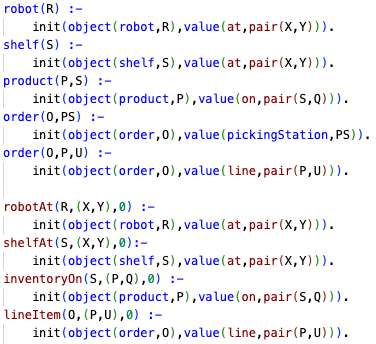
\includegraphics[width=0.9\columnwidth]{init.png}
\caption{Initial state}
\label{fig1:image}
\end{figure}

The primary challenges with this project was to represent the scenario as a program with a reasonable starting search space. In the following sections, there is heavy focus on grounding, generative axioms, and their effects on constraints and satisfiability of the program.

\subsection{Instantiation and Ground Terms}

The warehouse program is initialized with a given instance, which instantiates a set of ground terms that represent the starting state of the warehouse. As shown in Figure \ref{fig1:image}, this includes constant objects as well as fluents that represent the state of the world at time \ct{T=0}. This set of ground terms are the basis for generating our program's search space.

There are several instance rules that propagate both a constant object and a fluent, such as \ct{robot(R)} and \ct{robotAt(R,(X,Y),0)}. In order to minimize complexity and simplify rules and constraints of the program, symbolic constants are declared separately from their fluent counterparts.

For example, consider the \ct{carrying} fluent declared in terms of \ct{robotAt(R,(X,Y),T)} and \ct{shelfAt(S,(X,Y),T)} fluents rather than symbolic constants \ct{robot(R)} and \ct{shelf(S)}. In order to ground the term, all variables must be replaced with values. Although the fluents contain values \ct{(R,S)}, they also introduce irrelevant variables \ct{X,Y}, cause confusion with the time step value \ct{T} occurring in all three fluents, and possibly overlap with intentional, well-formed rules or constraints.

\begin{figure}[t]
    \centering
    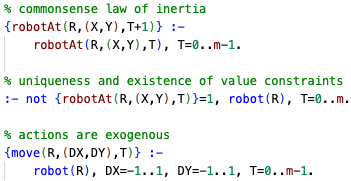
\includegraphics[width=0.8\columnwidth]{axiom.png}
    \caption{Domain independent axioms}
    \label{fig2:image}
    \end{figure}

\subsection{Domain Independent Axioms and Choice Rules}

Given a starting state, commonsense law of inertia states that the value of a fluent remains the same from one time step to the next, unless it is affected by an action or forced to change by another rule. Using choice rules, this is represented as
\begin{quote}\begin{small}\begin{verbatim}
{val of fluent(T+1)} :- val of fluent(T)
\end{verbatim}\end{small}\end{quote}
where \ct{\{...\}} denotes the set of choices, and the fluent has the option to keep its previous value. The choice rule allows this flexibility, where the fluent can take on a \emph{default} value in the absence of any other rules that influence the fluent. For example, the position of a robot should remain the same from one time step to the next, unless it is affected by a move action.

To enforce uniqueness and existence of fluents, we use choice rules to declare that there can only exist exactly one choice for each fluent, at each time step. This is expressed as \ct{1\{fluent(T)\}1} where the leftmost \ct{1} denotes that \emph{at least} one element must be chosen, and the rightmost \ct{1} denotes that \emph{at most} one element must be chosen. Constraints of this form are termed \emph{cardinality constraints}, where the number of choices are bounded. In this case, the cardinality constraint ensures that there exists exactly one choice for each fluent at each time step and is equivalently declared as \ct{\{fluent(T)\}=1}.

Note that on its own, the law of inertia does not guarantee that a robot's position will exist in the next time step since there is no lower bound on the choice rule. With the addition of the cardinality constraint, the law of inertia is enforced, and a robot \emph{must} stay in its previous position unless moved.

Expressing this as a constraint, any solution that satisfies the negated rule \ct{not \{fluent(T)\}=1}, violates the constraint, and is removed from the program's search space. This double negation semantic is referred to as \emph{negation as failure}. The intuition is that a rule is assumed false, unless there is evidence that it is true. That is, solutions are assumed not to violate a constraint, unless it is proven to violate the constraint. In our scenario, solutions where a robot does not have a unique position at each time step is eliminated as an answer set, effectively ensuring that plans will have robots placed at unique positions at each time step.

The exogenous nature of actions can also be declared using choice rules. Together with the ground terms of the starting state, the election of actions generate the program's search space with all possible sequences of actions that can occur in the world, as well as the resulting state of the world after each action. For the warehouse, this axiom that declares actions to be exogenous essentially populates the universe of warehouse states from the initial warehouse state by generating the set of all possible sequence of actions.

Consider Figure \ref{fig2:image} where the move action is declared as exogenous using an unbounded choice rule. The expression also specifies that \ct{R} is ground via \ct{robot(R)} and variables \ct{DX,DY} ranges over values (-1,0,1). In a single time step, there are 9 possible moves for each robot, resulting in 9! sequences of moves to add to the program's search space. While grounding this rule is simple, it can be challenging to ground more complex actions like \ct{deliver}.

\subsection{Effects and Preconditions of Actions}

The \ct{deliver} action is the most challenging to represent, with its subtle preconditions and nuanced effect on the \ct{inventoryOn} and \ct{lineItem} fluents. For the sake of completeness, we will briefly touch on the other actions before diving into the \ct{deliver} action.

\subsubsection{Move}

This action affects positional fluents, and its effect on the \ct{robotAt} is declared recursively. Any solutions where \ct{|DX|=|DY|} are diagonal or stationary, and removed from the search space. We also disallow two robots to swap positions.

Shelves can be relocated by moving robots carrying shelves, and this is expressed recursively with the added conditions on the \ct{carrying} fluent.

Other conflicting effects can be represented as state constraints, such as ensuring that the destination of a move is within the grid. This is represented as constraint that robots cannot be positioned on a non-node. Cardinality constraints are used to disallow two or more robots nor two or more shelves to occupy the same node and the same time. These rules also covers the cases where the effect of the move action may land either object on a node occupied by its like.

\subsubsection{Pick up \& Put down}

These two actions affect the \ct{carrying(B,(R,S),T)} fluent, and their effect can be declared recursively. The pick up action sets the carrying state to true for \ct{(R,S)} provided that the is located at the same node, and \ct{R} is not presently carrying a shelf. Conversely, the put down action sets the carrying state to false for \ct{(R,S)}, provided that \ct{R} is presently carrying  \ct{S}, and they are not located on a highway node.

\subsubsection{Deliver}

\begin{figure}[t]
    \centering
    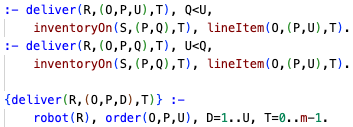
\includegraphics[width=0.9\columnwidth]{deliver.png}
    \caption{Deliver action}
\label{fig3:image}
\end{figure}

The fluents \ct{inventoryOn(S,(P,Q),T)} and \ct{lineItem(O,(P,U),T)} are affected by the \ct{deliver(R,(O,P,D),T)} action, whereby the inventory quantity \ct{Q}, and line item units \ct{U}, are decreased by \ct{D} number of products delivered. This effect is expressed recursively for both fluents. To ensure that the remaing inventory \ct{(Q-D)} and fulfillable line items \ct{(U-D)} do not fall below zero after the deliver action, the intuition is that delivered units \ct{D} must be the lesser of the two values:

\begin{enumerate}
    \item if \ct{Q>=U}, then \ct{D=U} to prevent \textit{over delivery}
    \item if \ct{U>=Q}, then \ct{D=Q} to prevent \textit{owing inventory}
\end{enumerate}

Consider the rule that declares the deliver action as exogenous. Grounding variables \ct{R,O,P,T} is trivial, but the domain of \ct{D} is not evident. The purpose of deliveries is to fulfill all line items of orders, and thus the lower bound of \ct{D} is set as 1 and the upper bound is the \emph{initial} number of units ordered. This is not necessarily the value of \ct{U} in \ct{lineItem(O,(P,U),T)}, that represents the \emph{remaining} number of units fulfillable at time step \ct{T}.

Recall the symbolic constant \ct{order\{O,P,U\}} in Figure \ref{fig1:image}. This represents the initial state of the order line item, and as seen in Figure \ref{fig3:image}, it becomes incredible useful in grounding the deliver action.

Figure \ref{fig3:image} also illustrates the constraints on \ct{D} is expressed as a negated form of conditions 1 and 2 listed above. More literally:

\begin{enumerate}
    \item[1'.] \textit{throw out plans that over deliver} - remove solutions with \ct{D=U} when \ct{Q<U} since constraint is violated
    \item[2'.] \textit{throw out plans that owe inventory} - remove solutions with \ct{D=Q} when \ct{U<Q} since constraint is violated
\end{enumerate}

Finally, we disallow deliveries to mismatched order picking stations, and ensure that robots are carrying the shelf that stocks the product in the order line item being delivered.

\subsection{Goal State and Objective Function}

\begin{figure}[t]
    \centering
    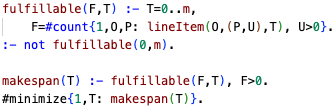
\includegraphics[width=0.9\columnwidth]{obj.png}
    \caption{Objective function}
\label{fig4:image}
\end{figure}

The goal state is defined as a warehouse with all orders fulfilled, that is, all line items in the final state of the scenario must have no remaining units to fulfill. Expressed as a constraint,

\begin{quote}\begin{small}\begin{verbatim}
:- not lineItem(O,(P,0),m), order(O,P,U).
\end{verbatim}\end{small}\end{quote}
where \ct{m} is the maximum time step.

Equivalently, the goal state must have no line items that remaining fulfillable units. We define the \ct{fulfillable(F,T)} aggregate to count \ct{F} number of line items with non-zero fulfillable units at time step \ct{T}. It follows that the \ct{makespan(T)} value is expressed in terms of the \ct{fulfillable} aggregate, the objective function is to minimize the makespan is demonstrated in Figure \ref{fig4:image}.

\begin{table*}[t]
    \centering
    \caption{Clingo Results}\smallskip
        \begin{tabular}{|c|c|c|c|c|c|c|} \hline
        Instance & Stations & Shelves & Products & Orders & Optimal Makespan & Solve Time (s) \\ \hline
        0 & 2 & 6 & 4 & 3 & 13 & 6.303 \\
        1 & 2 & 6 & 4 & 3 & 13 & 5.881 \\
        2 & 2 & 5 & 3 & 2 & 11 & 2.842 \\
        3 & 1 & 6 & 4 & 2 & 7 & 0.832 \\
        4 & 2 & 6 & 2 & 3 & 10 & 1.094 \\
        5 & 1 & 6 & 4 & 1 & 6 & 0.759 \\ \hline
        \end{tabular}
    \label{table1}
    \end{table*}

\section{Results and Analysis}

Using clingo, we solved the program initialized with the provided sample instances. In each case, the warehouse floor consisted of 16 nodes, 7 highways, and 2 robots. The maximum step size was set to 15 across all instances for consistency. The results are summarized in Table \ref{table1}, where \emph{Instance 0} denotes the example from the original problem description.


As the number of stations, shelves, products, and orders increase, the optimal makespan and solve time increases. This is expected since the program's search space increases with the number of objects and actions, and the number of possible sequences of actions increases exponentially with the number of time steps.

We can also review the performance of our program by replacing constraints with different representations that yield an optimal model of equivalent size. This provides insights on how changes in the representation of constraints may affect the program's search space, how effectively the solver can reduce the search space with a different representation, and the effects on solve time to finding an optimal model.

In the alternate programs illustrated in figure \ref{fig5:image}, we use initialize with Instance 0 and maximum step size 20. The original program takes 12.379s to find an optimal plan with a makespan of 13.

\begin{figure}[t]
    \centering
    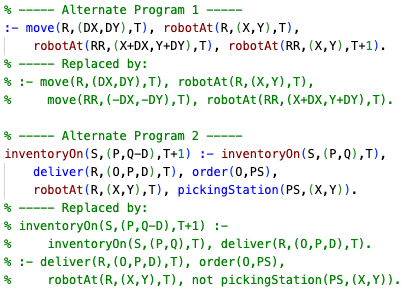
\includegraphics[width=0.9\columnwidth]{alternate.png}
    \caption{Alternate programs}
\label{fig5:image}
\end{figure}

\subsubsection{Alternate program 1}
The constraint for swapping positions is modified from having 1 action and 3 fluents, to 2 actions and 2 fluents. It takes clingo 35.649s to find an optimal plan with a makespan of 13. This is a significant increase in solve time, and the program is not as effective in reducing the search space.

\subsubsection{Alternate program 2}
The delivery effect on inventory is modified from having the designated picking station condition inline with the recursive definition, to expressing this as a separate constraint. It takes clingo 19.050s to find an optimal plan with a makespan of 13. Here we see that having constraints as part of the recursive definition is more effective in reducing the search space.

\section{Conclusion}

This project has been a great learning experience in applying answer set programming to a real-world scenario. Through trialing various representations, it has put into context theories and formalisms learned in lectures, and helped connect the dots between abstract concepts such as the implication of exogenous actions on the program search space. The project has been instrumental in gaining a deeper understanding of knowledge representation and reasoning in practice, and answer set programming and its applications.

\section{Opportunities for Future Work}

In the original scenario description, there is mention of permitting robots to perform multiple concurrent actions at each time step. This would involve modifying the program to generate only serializable plans, where actions that are scheduled for the same time step can be executed in any order, without affecting the result. It would be interesting to explore the changes to satisfability and optimality in the modified program.

\nocite{found}
\nocite{recon}
\nocite{reform}
\nocite{glimpse}
\nocite{kaufmann2016grounding}
\nocite{Lifschitz2016AnswerSA}
\nocite{inproceedings}

\begin{quote}
    \begin{small}
        \bibliographystyle{aaai}
        \bibliography{references}
    \end{small}
\end{quote}
\end{document}
